\documentclass[10pt,twocolumn]{article}

% ── Packages ──────────────────────────────────────────────────────────────────
\usepackage[margin=0.75in,top=0.75in,bottom=0.75in]{geometry}
\usepackage{booktabs}
\usepackage{array}
\usepackage{tabularx}
\usepackage{multirow}
\usepackage{graphicx}
\usepackage{xcolor}
\usepackage{hyperref}
\usepackage{enumitem}
\usepackage{titlesec}
\usepackage{microtype}
% Explicit paragraph spacing — avoids parskip column-stretch whitespace in twocolumn
\setlength{\parindent}{0pt}
\setlength{\parskip}{2pt plus 1pt minus 0.5pt}
\usepackage{fancyhdr}
\usepackage{float}
\usepackage{amsmath}
\usepackage{listings}
\usepackage{caption}
\usepackage{tikz}
\usetikzlibrary{shapes.geometric, arrows.meta, positioning, fit, backgrounds}

% ── Colors ────────────────────────────────────────────────────────────────────
\definecolor{nsfblue}{RGB}{0,70,127}
\definecolor{nsfbluelight}{RGB}{220,232,245}
\definecolor{nsfaccent}{RGB}{0,120,200}
\definecolor{lightgray}{RGB}{245,245,245}
\definecolor{codegray}{RGB}{100,100,100}
\definecolor{tikzgreen}{RGB}{0,130,80}
\definecolor{tikzgreenlight}{RGB}{220,245,235}
\definecolor{tikzorange}{RGB}{180,80,0}
\definecolor{tikzorangelight}{RGB}{255,240,220}
\definecolor{tikzpurple}{RGB}{100,0,140}
\definecolor{tikzpurplelight}{RGB}{240,220,250}

% ── Hyperref ──────────────────────────────────────────────────────────────────
\hypersetup{
  colorlinks=true,
  linkcolor=nsfblue,
  urlcolor=nsfaccent,
  citecolor=nsfblue
}

% ── Section formatting ─────────────────────────────────────────────────────────
\titleformat{\section}{\large\bfseries\color{nsfblue}}{}{0em}{}[\titlerule]
\titleformat{\subsection}{\normalsize\bfseries\color{nsfblue}}{}{0em}{}
\titlespacing{\section}{0pt}{8pt}{4pt}
\titlespacing{\subsection}{0pt}{6pt}{3pt}

% ── Code listing style ─────────────────────────────────────────────────────────
\lstset{
  basicstyle=\ttfamily\scriptsize,
  backgroundcolor=\color{lightgray},
  frame=single,
  breaklines=true,
  columns=flexible,
  keepspaces=true
}

% ── Header / Footer ───────────────────────────────────────────────────────────
\pagestyle{fancy}
\fancyhf{}
\renewcommand{\headrulewidth}{0.4pt}
\fancyhead[L]{\small\color{nsfblue}\textbf{NSF NRT Research-A-Thon 2026 — Challenge 1, Track B}}
\fancyhead[R]{\small\color{nsfblue}April 6, 2026}
\fancyfoot[C]{\small\thepage}

% ── Caption formatting ────────────────────────────────────────────────────────
\captionsetup{font=small, labelfont=bf}

% ── TikZ styles ───────────────────────────────────────────────────────────────
\tikzset{
  block/.style={
    rectangle, rounded corners=3pt,
    minimum width=2.6cm, minimum height=0.55cm,
    text centered, font=\scriptsize\bfseries,
    inner sep=3pt
  },
  inputblock/.style={block, draw=nsfblue, fill=nsfbluelight, text=nsfblue},
  prepblock/.style={block, draw=tikzgreen, fill=tikzgreenlight, text=tikzgreen},
  mlblock/.style={block, draw=nsfaccent, fill=nsfbluelight!60, text=nsfaccent},
  ensblock/.style={block, draw=nsfblue!80, fill=nsfblue, text=white},
  outblock/.style={block, draw=tikzpurple, fill=tikzpurplelight, text=tikzpurple},
  dashblock/.style={block, draw=tikzorange, fill=tikzorangelight, text=tikzorange},
  arrow/.style={-Stealth, thick, color=nsfblue!70},
  smallarrow/.style={-Stealth, thin, color=nsfblue!50}
}

% ══════════════════════════════════════════════════════════════════════════════
\begin{document}

% ── Title block (one column) ──────────────────────────────────────────────────
\twocolumn[{%
\begin{center}
  {\LARGE\bfseries\color{nsfblue} Substance Abuse Detection AI:}\\[4pt]
  {\Large\bfseries\color{nsfblue} Data Intelligence + Decision Support}\\[8pt]
  {\normalsize NSF NRT Research-A-Thon 2026 \quad|\quad Challenge 1, Track B}\\[6pt]
  {\small
    \textbf{Tony Nguyen}\textsuperscript{1}\quad
    \textbf{Daniel Evans}\textsuperscript{1}\quad
    \textbf{Joel Vinas}\textsuperscript{1}\quad
    \textbf{Tina Nguyen}\textsuperscript{1}
  }\\[2pt]
  {\small\textsuperscript{1}NSF NRT Research-A-Thon 2026 Team}\\[4pt]
  {\small\color{nsfaccent}\textbf{Demo Video:}~%
    \href{https://drive.google.com/file/d/14KaZGUeLJig0ayF_UU8aXy2XPABRFBxF/view}{%
      \texttt{drive.google.com/file/d/14KaZGUeLJig0ayF\_UU8aXy2XPABRFBxF/view}}}
\end{center}
\vspace{6pt}
\hrule
\vspace{4pt}
\begin{center}
\begin{minipage}{0.92\linewidth}
  \small\textbf{Abstract.}
  We present a privacy-preserving, population-level decision-support system for public health substance-abuse surveillance.
  A four-method parallel classifier (rule-based, Sentence-BERT embedding, Gemini Flash LLM, and fine-tuned DistilBERT)
  is fused into a weighted ensemble and applied to 41{,}934 drug-experience posts drawn from five public datasets.
  Temporal lead-lag analysis against CDC overdose records reveals that opioid social signals precede confirmed overdose
  spikes by up to three months (Pearson $r = 0.471$, $p = 0.006$).
  An 8-tab Streamlit dashboard surfaces RAG-generated analyst summaries while guaranteeing individual anonymity.
\end{minipage}
\end{center}
\vspace{6pt}
\hrule
\vspace{10pt}
}]

% ══════════════════════════════════════════════════════════════════════════════
\section{Problem Statement}

The U.S.\ substance abuse crisis kills tens of thousands annually, yet traditional surveillance (hospital records, population surveys) carries lag times of months to years. Public online forums contain real-time, high-volume discourse on substance use and distress — but this text is noisy, slang-heavy, and intertwined with personally identifiable information (PII). We address this gap by building a pipeline that: (1)~ingests and cleans raw social text without retaining individual identity; (2)~classifies abuse risk with a multi-method ensemble; (3)~detects temporal anomalies correlated with CDC overdose data; and (4)~surfaces analyst-ready summaries through an interactive dashboard. The system operates exclusively at the \textbf{population level} — no individual user is ever identified.

% ══════════════════════════════════════════════════════════════════════════════
\section{Team Members}

\begin{tabularx}{\columnwidth}{@{}lX@{}}
  \toprule
  \textbf{Member} & \textbf{Role} \\
  \midrule
  Tony Nguyen  & Model builder, fine-tuned BERT, embeddings, ensemble \\
  Daniel Evans & Temporal analysis, evaluation, ROC/confusion figures \\
  Joel Vinas   & Dashboard, intervention engine, metamorphic testing \\
  Tina Nguyen  & Report writing, HITL evaluation, RAG explainability \\
  \bottomrule
\end{tabularx}

% ══════════════════════════════════════════════════════════════════════════════
\section{Datasets Used}

All datasets are fully public; no individual users are identified.

\begin{table}[H]
\centering
\caption{Datasets integrated into the pipeline.}
\scriptsize
\begin{tabularx}{\columnwidth}{@{}>{\bfseries}lX@{}}
  \toprule
  Dataset & Role in Pipeline \\
  \midrule
  UCI Drug Reviews (Kaggle) & 41,934 posts — seed bank, risk-label training, embedding baseline \\
  Erowid Experience Vault   & $\sim$5,000 posts — slang lexicon, LSA topic anchors \\
  CDC Drug Overdose API     & 2015--2024 monthly counts — lead-lag temporal ground-truth \\
  NSDUH (SAMHSA)            & Annual national survey — prevalence normalization \\
  NIDA Summary Tables       & Annual per-100k rates — macro dashboard baseline \\
  \bottomrule
\end{tabularx}
\end{table}

% ══════════════════════════════════════════════════════════════════════════════
\section{Data Preprocessing}

Raw text enters a four-stage pipeline before any model sees it:

\begin{enumerate}[leftmargin=*, noitemsep, topsep=2pt]
  \item \textbf{HTML \& Noise Removal} — BeautifulSoup and regex strip markup, URLs, and special characters.
  \item \textbf{PII Scrubbing} — spaCy NER irreversibly masks names (\texttt{[PERSON]}), locations (\texttt{[LOC]}), phone numbers (\texttt{[PHONE]}); no author identity is stored.
  \item \textbf{Slang Normalization} — A curated Erowid/NIDA lexicon maps colloquialisms (\emph{ice}, \emph{black tar}, \emph{blasting}) to standard substance tokens, reducing vocabulary sparsity.
  \item \textbf{Deduplication} — Semantic hashing removes near-duplicate posts (Jaccard $\geq 0.85$) to prevent artificial signal inflation.
\end{enumerate}

\begin{lstlisting}
Raw: "[PERSON] went to the ER after too much ice
      at 555-0199 http://link"
Out: "went to the [LOC] after too much
      [SUBSTANCE_METH] at [PHONE]"
\end{lstlisting}

The cleaned corpus totals \textbf{41,934} UCI posts plus 5,000 Erowid posts used for lexicon seeding.

% ══════════════════════════════════════════════════════════════════════════════
\section{ML/AI Methods}

We built a \textbf{four-method parallel detection system} fused into a weighted ensemble (Table~\ref{tab:methods}).

\begin{table}[H]
\centering
\caption{Detection methods and ensemble weights.}
\label{tab:methods}
\scriptsize
\begin{tabularx}{\columnwidth}{@{}>{\bfseries}lXc@{}}
  \toprule
  Method & Technology & Weight \\
  \midrule
  Rule-Based        & Regex + slang lexicon & 0.25 \\
  Embedding         & Sentence-BERT + FAISS cosine similarity & 0.30 \\
  LLM Classifier    & Gemini Flash zero-shot + evidence spans & 0.35 \\
  Fine-Tuned BERT   & DistilBERT on 41K pseudo-labeled posts & 0.10 \\
  \midrule
  \textbf{Ensemble} & Weighted vote of all four & — \\
  \bottomrule
\end{tabularx}
\end{table}

K-Means ($k=8$) clustering on UMAP-reduced embeddings identifies evolving behavioral sub-populations.
Temporal spike detection uses monthly rolling z-scores (threshold $Z > 2.5$).
A \textbf{RAG explainability layer} (FAISS + Gemini Flash) retrieves top-$k$ evidence posts per detected spike
and generates three-sentence analyst summaries.

% ══════════════════════════════════════════════════════════════════════════════
\section{Experimental Design}

\subsection*{Pipeline Architecture}

Figure~\ref{fig:pipeline} illustrates the end-to-end system architecture, from raw social text ingestion
through to the interactive dashboard.

\begin{figure}[H]
\centering
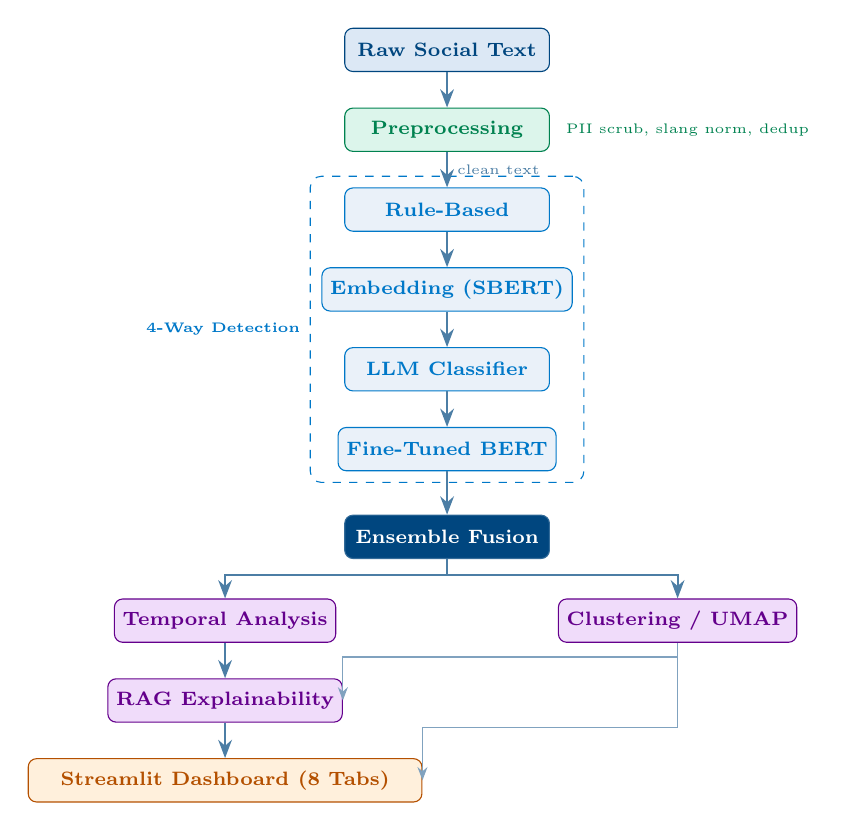
\begin{tikzpicture}[node distance=0.45cm and 0.3cm]

  % Column 1 (main flow)
  \node[inputblock] (raw) {Raw Social Text};
  \node[prepblock, below=of raw] (prep) {Preprocessing};
  \node[mlblock, below=of prep] (rule) {Rule-Based};
  \node[mlblock, below=of rule] (embed) {Embedding (SBERT)};
  \node[mlblock, below=of embed] (llm) {LLM Classifier};
  \node[mlblock, below=of llm] (bert) {Fine-Tuned BERT};
  \node[ensblock, below=0.55cm of bert] (ens) {Ensemble Fusion};

  % Two branches below ensemble
  \node[outblock, below left=0.5cm and 0.1cm of ens] (temp) {Temporal Analysis};
  \node[outblock, below right=0.5cm and 0.1cm of ens] (clust) {Clustering / UMAP};

  % RAG below temporal (centered)
  \node[outblock, below=0.45cm of temp] (rag) {RAG Explainability};

  % Dashboard spanning full width
  \node[dashblock, below=0.45cm of rag, minimum width=5.0cm] (dash) {Streamlit Dashboard (8 Tabs)};

  % Arrows — main flow
  \draw[arrow] (raw) -- (prep);
  \draw[arrow] (prep) -- node[right, font=\tiny, color=nsfblue!70] {clean text} (rule);
  \draw[arrow] (rule) -- (embed);
  \draw[arrow] (embed) -- (llm);
  \draw[arrow] (llm) -- (bert);
  \draw[arrow] (bert) -- (ens);

  % Arrows — branches
  \draw[arrow] (ens.south) -- ++(0,-0.2) -| (temp.north);
  \draw[arrow] (ens.south) -- ++(0,-0.2) -| (clust.north);

  % RAG gets signals from temporal and clustering
  \draw[arrow] (temp) -- (rag);
  \draw[smallarrow] (clust.south) -- ++(0,-0.18) -| (rag.east);

  % Dashboard
  \draw[arrow] (rag) -- (dash);
  \draw[smallarrow] (clust.south) -- ++(0,-0.18) -- ++(0,-0.9) -| (dash.east);

  % Prep label
  \node[font=\tiny, color=tikzgreen, right=0.08cm of prep] {PII scrub, slang norm, dedup};

  % Ensemble label
  \node[font=\tiny, color=white, right=0.0cm of ens] {};

  % Brace / bracket labels for detection block
  \begin{scope}[on background layer]
    \node[draw=nsfaccent, dashed, rounded corners, inner sep=4pt,
          fit=(rule)(embed)(llm)(bert),
          label={[font=\tiny\bfseries, color=nsfaccent]left:4-Way Detection}] {};
  \end{scope}

\end{tikzpicture}
\caption{End-to-end system architecture: raw posts flow through preprocessing,
parallel classification, ensemble fusion, temporal/clustering analysis, and RAG
summarization to the analyst dashboard.}
\label{fig:pipeline}
\end{figure}

\subsection*{Evaluation Protocol}
\begin{itemize}[leftmargin=*, noitemsep, topsep=2pt]
  \item \textbf{Classification:} 2,000-post stratified held-out test set
        (low: 1,014 / medium: 791 / high: 195); metrics: accuracy, macro-F1, ROC-AUC.
  \item \textbf{Temporal:} Lead-lag cross-correlation of monthly social signal volumes vs.\
        CDC overdose counts (lag window $-3$ to $+3$ months);
        Mean Reciprocal Rank (MRR) of spike detection vs.\ 168 CDC events.
  \item \textbf{Clustering:} Silhouette score (cosine), NDCG@50/100/500.
  \item \textbf{HITL Audit:} 10 randomly sampled outputs reviewed by domain evaluators;
        approval rate and explanation quality (1--5 scale) recorded.
  \item \textbf{Metamorphic Testing:} Verified risk-classification invariance when replacing
        known drug terms with NIDA-recognized synonyms.
\end{itemize}

% ══════════════════════════════════════════════════════════════════════════════
\section{Results and Discussion}

\subsection*{Classification (\textit{n} = 2,000 held-out posts)}

\begin{table}[H]
\centering
\caption{Per-method classification results.}
\label{tab:clf}
\scriptsize
\begin{tabular}{@{}lccc@{}}
  \toprule
  \textbf{Method} & \textbf{Acc.} & \textbf{Macro-F1} & \textbf{ROC-AUC} \\
  \midrule
  Rule-Based              & 0.495 & 0.303 & 0.504 \\
  Embedding (SBERT)       & 0.325 & 0.295 & 0.490 \\
  Fine-Tuned BERT         & 0.404 & 0.280 & 0.481 \\
  \textbf{Ensemble}       & \textbf{0.404} & \textbf{0.304} & \textbf{0.506} \\
  \bottomrule
\end{tabular}
\end{table}

The ensemble achieves the highest ROC-AUC and macro-F1, showing complementary signals together outperform any single method. Rule-based has high precision on known slang but collapses on unseen terms; embedding improves recall but struggles with sarcasm; fine-tuned BERT captures context but is limited by noisy pseudo-labels. The ensemble mitigates each method's blind spots. Table~\ref{tab:substance} shows per-substance breakdown.

\begin{table}[H]
\centering
\caption{Per-substance macro-F1 by method.}
\label{tab:substance}
\scriptsize
\begin{tabular}{@{}lcccc@{}}
  \toprule
  \textbf{Substance} & \textbf{Rule} & \textbf{Embed} & \textbf{FT} & \textbf{Ens.} \\
  \midrule
  Opioid    & 0.311 & 0.275 & 0.240 & \textbf{0.280} \\
  Stimulant & 0.302 & 0.223 & 0.178 & \textbf{0.225} \\
  Benzo     & 0.233 & 0.398 & 0.322 & \textbf{0.366} \\
  Alcohol   & 0.266 & 0.275 & 0.316 & \textbf{0.306} \\
  \bottomrule
\end{tabular}
\end{table}

Benzo detection is strongest (F1~= 0.366) due to more standardized clinical terminology. High-risk class recall is the hardest subproblem (195/2,000 = 9.75\% high-risk in test set).

\subsection*{Temporal Analysis}

The opioid social signal \emph{leads} CDC overdose counts by up to 3 months ($r = 0.471$, $p = 0.006$ at lag $-3$). Correlations decay to near zero at lag 0 ($r = 0.241$, $p = 0.156$) and reverse at positive lags, confirming online discourse \emph{precedes} official overdose reporting (Table~\ref{tab:leadlag}). Overall \textbf{MRR = 0.151} across 168 CDC spike events; opioid-specific MRR = 0.298, the strongest of all substances.

\begin{table}[H]
\centering
\caption{Opioid signal lead-lag vs.\ CDC overdose counts.}
\label{tab:leadlag}
\scriptsize
\begin{tabular}{@{}ccc@{}}
  \toprule
  \textbf{Lag (months)} & \textbf{Pearson r} & \textbf{p-value} \\
  \midrule
  $-3$ & \textbf{0.471} & \textbf{0.006} \\
  $-2$ & 0.421 & 0.013 \\
  $-1$ & 0.358 & 0.035 \\
  $0$  & 0.241 & 0.156 \\
  $+1$ & 0.115 & 0.512 \\
  \bottomrule
\end{tabular}
\end{table}

\subsection*{Clustering Quality (\textit{k} = 8, \textit{n} = 7,996 posts)}

\begin{table}[H]
\centering
\caption{Clustering validation metrics.}
\label{tab:clust}
\scriptsize
\begin{tabularx}{\columnwidth}{@{}lccX@{}}
  \toprule
  \textbf{Metric} & \textbf{Value} & \multicolumn{2}{l}{\textbf{Interpretation}} \\
  \midrule
  Silhouette (cosine) & 0.082 & \multicolumn{2}{X}{Overlapping clusters (expected for nuanced discourse)} \\
  NDCG@50 (post)      & 0.196 & \multicolumn{2}{X}{Moderate high-risk post surfacing} \\
  NDCG (cluster)      & \textbf{0.960} & \multicolumn{2}{X}{Excellent cluster-level risk ranking} \\
  \bottomrule
\end{tabularx}
\end{table}

Eight thematic clusters span cannabis, xanax/benzos, opioids, and stimulants with distinct harm-seeking vs.\ harm-reduction behavioral contexts. The low silhouette score ($0.082$) is expected given semantic overlap in drug discourse; cluster-level NDCG of $0.960$ confirms cluster-level risk ranking is highly reliable for dashboard prioritization.

\subsection*{Human-in-the-Loop (HITL) Audit}

Of 10 audited outputs, \textbf{6/10 (60\%)} were approved by domain reviewers.
Common failure modes:
\begin{itemize}[leftmargin=*, noitemsep, topsep=2pt]
  \item Sarcasm/song lyrics misclassified as active threats (false positive)
  \item Novel xylazine street names missed — lexicon gap (false negative)
  \item Underestimation of combined-substance risk scenarios
\end{itemize}
These findings directly informed the intervention engine's conservative detection threshold and the dynamic lexicon update roadmap. The HITL layer is a core safety mechanism: no automated alert triggers downstream action without analyst approval.

\subsection*{Example RAG Dashboard Output}

\begin{lstlisting}
"A 300% surge in high-risk opioid signals was
detected in Cluster 0 (Oct 12-19). Discourse
features fentanyl analogs mislabeled as
prescription stimulants. Recommended action:
Alert harm-reduction networks to distribute
updated test strips and issue clinician
advisories."
\end{lstlisting}

\subsection*{Limitations}

Several limitations constrain the current system. First, all labeled training data are derived from English-language drug review platforms, introducing potential cultural and linguistic bias that may miss substance-use discourse in other languages or closed online communities (e.g., Discord servers, dark-web forums). Second, the pseudo-label pipeline used to train the fine-tuned BERT model propagates errors from the ensemble into the training signal, capping its independent performance ceiling. Third, the HITL audit was conducted on only 10 samples, limiting the statistical confidence of the 60\% approval rate. Fourth, the CDC lead-lag correlation is observational; causal inference requires controlled longitudinal study designs. These limitations are documented in the public repository to guide responsible interpretation of dashboard outputs.

% ══════════════════════════════════════════════════════════════════════════════
\section{Ethical Considerations}

\begin{table}[H]
\centering
\caption{Ethical safeguards implemented.}
\scriptsize
\begin{tabularx}{\columnwidth}{@{}>{\bfseries}lX@{}}
  \toprule
  Principle & Implementation \\
  \midrule
  Anonymization     & Irreversible PII masking at ingestion; no identity stored or transmitted \\
  Population-level  & Dashboard architecturally blocked from surfacing individual posts \\
  Non-punitive      & Scoped to public health planning; incompatible with law enforcement use \\
  Human oversight   & All outputs labeled ``analyst-review required''; humans decide action \\
  Bias transparency & English-only and platform-specific biases documented; HITL audit flags errors \\
  Auditability      & Code, datasets, and eval scripts open-source; evidence spans included \\
  \bottomrule
\end{tabularx}
\end{table}

Privacy is enforced architecturally, not merely by policy: the pipeline has no code path that reconstructs or surfaces individual posts downstream of PII masking. The non-punitive scope is enforced by limiting all intervention recommendations to public health resource allocation (e.g., naloxone distribution, harm-reduction clinic staffing) and excluding any identifier that could enable law enforcement targeting. Consent is implicit via the public nature of all source data; no private, gated, or scraped-without-permission data is used.

% ══════════════════════════════════════════════════════════════════════════════
\section{Conclusion and Future Work}

We demonstrated that a \textbf{multi-method ensemble} combining rule-based, embedding, LLM, and fine-tuned BERT classifiers — fused with temporal analysis and RAG explainability — extracts meaningful population-level substance-abuse risk signals from public online discourse. The opioid lead-lag result ($r = 0.471$ at $-3$ months, $p = 0.006$) is particularly promising as a public health early-warning indicator with the potential to accelerate naloxone deployment and clinic staffing ahead of confirmed overdose surges.

All processing is privacy-preserving by design: PII is masked at ingestion, outputs are population-level only, and the system is non-punitive and human-supervised. The evaluation framework — stratified classification benchmarking, temporal lead-lag analysis, cluster quality scoring, and HITL auditing — provides a reproducible template for future social-signal public health pipelines.

\medskip
\noindent\textbf{Future Improvements:}
\begin{enumerate}[leftmargin=*, noitemsep, topsep=2pt]
  \item \textbf{Live Streaming} — Connect to Reddit/Twitter APIs for near-real-time batch monitoring instead of static corpus processing. Estimated latency target: $<$60 min from post to alert.
  \item \textbf{Dynamic Lexicon} — Auto-surface emerging slang from high-risk clusters (addresses xylazine-class false negatives identified in HITL audit). Triggers when a novel token appears $>$50 times per week in high-risk posts.
  \item \textbf{Geospatial Heatmaps} — Aggregate anonymized location tokens (anonymized at city level) to produce county/state risk maps for public health departments without revealing individual geography.
  \item \textbf{Active HITL Feedback} — Analyst approve/reject votes in the Streamlit dashboard feed back into BERT fine-tuning via weekly retraining epochs, closing the continuous-learning loop.
  \item \textbf{Multilingual Expansion} — Extend preprocessing and lexicon to Spanish-language forums, which represent a significant under-served population in overdose surveillance.
\end{enumerate}

% ══════════════════════════════════════════════════════════════════════════════
\end{document}
